\chapter{函数}

\section{函数}

\subsection{函数(Function)}

函数执行一个特定的任务,Python提供了大量内置函数,例如print()用来输出字符串、len()用来计算序列长度等。

\begin{figure}[H]
	\centering
	\begin{tikzpicture}[scale=0.5]
		\draw[-] (5,-2) -- (10,-2) -- (10,2) -- (5,2) -- (5,-2);
		\draw[->] (0,0) -- (5,0);
		\draw[->] (10,0) -- (15,0);

		\draw (-2,0) node {Input};
		\draw (17,0) node {Output};
		\draw (7.5,0) node {Function};
	\end{tikzpicture}
	\caption{函数}
\end{figure}

当调用函数时,程序控制权会转移给被调用的函数,当函数执行结束后,函数会把程序序控制权交还给其调用者。

\begin{figure}[H]
	\centering
	\begin{tikzpicture}[]
		\draw (0,4.5) node {Caller};
		\draw[->] (0,4) -- (0,0.5);
		\draw[->] (0,-0.5) -- (0,-4);
		\draw (0,0) node {调用foo()};

		\draw (4,4) node {foo()};
		\draw[->] (4,3) -- (4,0.5);
		\draw[->] (4,-0.5) -- (4,-3);
		\draw (4,0) node {调用bar()};

		\draw (8,3) node {bar()};
		\draw[->] (8,2) -- (8,-2);

		\draw[->] (0.5,0.5) -- (3.5,3);
		\draw[->] (3.5,-3) -- (0.5,-0.5);
		\draw[->] (4.5,0.5) -- (7.5,2);
		\draw[->] (7.5,-2) -- (4.5,-0.5);
	\end{tikzpicture}
	\caption{函数调用}
\end{figure}

使用def关键字可以定义函数:

\vspace{-0.5cm}

\begin{lstlisting}[language=Python]
def func_name([param_list]):
    # code
\end{lstlisting}

\vspace{0.5cm}

\subsection{函数设计方法}

为什么不把所有的代码全部写在一起,还需要自定义函数呢?\\

使用函数有以下好处:

\begin{enumerate}
	\item 避免代码复制,代码复制是程序质量不良的表现
	\item 便于代码维护
	\item 避免重复造轮子,提高开发效率
\end{enumerate}

在设计函数的时候需要考虑以下的几点要素:

\begin{enumerate}
	\item 确定函数的功能

	\item 确定函数的参数
	      \begin{itemize}
		      \item 是否需要参数
		      \item 参数个数
		      \item 参数类型
	      \end{itemize}

	\item 确定函数的返回值
	      \begin{itemize}
		      \item 是否需要返回值
		      \item 返回值类型
	      \end{itemize}
\end{enumerate}

\mybox{函数实现返回最大值}

\begin{lstlisting}[language=Python]
def get_max(num1, num2):
    # if num1 > num2:
    #     return num1
    # else:
    #     return num2

    return num1 if num1 > num2 else num2

print(get_max(4, 12))
print(get_max(54, 33))
print(get_max(0, -12))
print(get_max(-999, -774))
\end{lstlisting}

\begin{tcolorbox}
	\mybox{运行结果}
	\begin{verbatim}
12
54
0
-774
\end{verbatim}
\end{tcolorbox}

\vspace{0.5cm}

\mybox{函数实现累加和}

\begin{lstlisting}[language=Python]
def get_sum(start, end):
    total = 0
    for i in range(start, end+1):
        total += i
    return total

print("1-100的累加和 = %d" % get_sum(1, 100))
print("1024-2048的累加和 = %d" % get_sum(1024, 2048))
\end{lstlisting}

\begin{tcolorbox}
	\mybox{运行结果}
	\begin{verbatim}
1-100的累加和 = 5050
1024-2048的累加和 = 1574400
\end{verbatim}
\end{tcolorbox}

\vspace{0.5cm}

\mybox{函数实现输出i行j列由自定义字符组成的图案}

\begin{lstlisting}[language=Python]
def print_chars(row, col, c):
    for i in range(row):
        for j in range(col):
            print(c, end='')
        print()

print_chars(5, 10, '?')
\end{lstlisting}

\begin{tcolorbox}
	\mybox{运行结果}
	\begin{verbatim}
??????????
??????????
??????????
??????????
??????????
\end{verbatim}
\end{tcolorbox}

\newpage

\section{主函数}

\subsection{主函数}

Python是为数不多的直接定义完源代码就可以执行的编程语言,很多编程语言对于程序的执行都有非常严格的标准,例如C、C++、Java等都有主函数(主方法)来标记程序的起点。\\

在现实的开发之中主函数是很有必要的,可以区分出其它的结构,在模块中更需要主函数的使用。\\

在Python中如果想实现主函数的定义,必须借助于全局变量\_\_name\_\_的返回内容,而后采用自定义的函数形式实现,返回的\_\_main\_\_是一个字符串,这个内容是会改变的,跟程序身处的结构有关。\\

在很多的编程语言都将主函数通过main这个标识符来定义,所以定义的main()是符合一般的习惯的。在进行复杂开发的时候,强烈建议使用主函数作为程序的起点。\\

\mybox{主函数}

\begin{lstlisting}[language=Python]
def main():
    pass

if __name__ == "__main__":
    main()
\end{lstlisting}

\newpage

\section{变量作用域}

\subsection{变量作用域}

一个变量会根据其自身所处的位置由不同的作用范围,不同范围内使用的变量采用就近取用的原则。\\

Python的变量作用域采用LEGB原则:

\begin{itemize}
	\item Local:函数内部变量名称。
	\item Enclosing Function Locals:外部嵌套函数变量名称。
	\item Global:函数所在模块或程序文件的变量名称。
	\item Builtin:内置模块的变量名称。
\end{itemize}

\begin{figure}[H]
	\centering
	\begin{tikzpicture}[]
		\draw (4,4.5) node {全局};
		\draw (0,0) rectangle (8,4);

		\draw (2.5,3.5) node {局部};
		\draw (1,1) rectangle (4,3);

		\draw (2.5,2.5) node {变量A};
		\draw (2,1.5) rectangle (3,2);

		\draw (6,2.5) node {变量B};
		\draw (5.5,1.5) rectangle (6.5,2);
	\end{tikzpicture}
	\caption{变量作用域}
\end{figure}

在一个Python源文件之中可以存在有若干个函数(或者类),每一个函数里面有可能定义自己的变量,但是这个变量不是公共的。局部变量只能被一个函数所使用的,其它的函数都无法进行操作。\\

\mybox{局部变量}

\begin{lstlisting}[language=Python]
def foo():
	num = 123

def main():
	print(num)

if __name__ == "__main__":
	main()
\end{lstlisting}

\begin{tcolorbox}
	\mybox{运行结果}
	\begin{verbatim}
NameError: name 'num' is not defined
\end{verbatim}
\end{tcolorbox}

如果希望在函数中访问全局的变量,可以通过global关键字实现。\\

\mybox{全局变量}

\begin{lstlisting}[language=Python]
num = 123	   # 全局变量

def foo():
	num = 321   # 局部变量
	print("foo(): %d" % num)	# 321

def bar():
	global num  # 调用全局变量
	num = 456
	print("bar(): %d" % num)	# 456

def main():
	foo()
	print(num)  # 123
	bar()
	print(num)  # 456

if __name__ == "__main__":
	main()
\end{lstlisting}

\begin{tcolorbox}
	\mybox{运行结果}
	\begin{verbatim}
foo(): 321
123
bar(): 456
456
\end{verbatim}
\end{tcolorbox}

\newpage

\section{函数参数}

\subsection{参数默认值}

在进行函数参数定义的时候,也可以设置默认值。当参数没有传递的时候就利用默认值来进行参数内容的填充,如果在参数上定义了默认值,那么该参数一定要放在参数列表的最后。\\

\mybox{参数默认值}

\begin{lstlisting}[language=Python]
def set_date(year=1970, month=1, day=1):
	print("%04d-%02d-%02d" % (year, month, day))

def main():
	set_date(2021, 4, 1)
	set_date(2021, 3)
	set_date(2021)
	set_date()

if __name__ == "__main__":
	main()
\end{lstlisting}

\begin{tcolorbox}
	\mybox{运行结果}
	\begin{verbatim}
2021-04-01
2021-03-01
2021-01-01
1970-01-01
\end{verbatim}
\end{tcolorbox}

\vspace{0.5cm}

\subsection{可变参数}

在Python中提供有可变参数形式,所有可变参数都使用元组进行接收。\\

\mybox{可变参数}

\begin{lstlisting}[language=Python]
def calculate(operator, *nums):
	"""
		定义一个可变参数的数学计算
		通过传入的运算符和运算数进行计算
		Args:
			operator (str): 运算符
			nums (tuple): 运算数(可变参数)
		Return:
			计算结果
	"""
	if operator == '+':
		result = 0
		for num in nums:
			result += num
	elif operator == '*':
		result = 1
		for num in nums:
			result *= num
	return result

def main():
	print("累加:%d" % calculate('+', 1, 2, 3, 4, 5))
	print("阶乘:%d" % calculate('*', 1, 2, 3, 4, 5))

if __name__ == "__main__":
	main()
\end{lstlisting}

\begin{tcolorbox}
	\mybox{运行结果}
	\begin{verbatim}
累加:15
阶乘:120
\end{verbatim}
\end{tcolorbox}

在进行参数传递的时候也可以使用【**】来标记关键字参数(字典)。\\

\mybox{关键字参数}

\begin{lstlisting}[language=Python]
def print_scores(name, **scores):
	print(name)
	for key, value in scores.items():
		print("\t|- %s: %s" % (key, value))

def main():
	print_scores("小灰", Python=100, Java=95)
	print_scores("小白", 数据结构=78, 算法=82)

if __name__ == "__main__":
	main()
\end{lstlisting}

\begin{tcolorbox}
	\mybox{运行结果}
	\begin{verbatim}
小灰
    |- Python: 100
    |- Java: 95
小白
    |- 数据结构: 78
    |- 算法: 82
\end{verbatim}
\end{tcolorbox}

\newpage

\section{lambda表达式}

\subsection{lambda表达式}

lambda指的是函数式编程,函数式编程最简单的理解就是没有名字的函数。lambda定义简单,只使用一次。

\vspace{-0.5cm}

\begin{lstlisting}[language=Python]
lambda param1, param2, ...: statement
\end{lstlisting}

一般而言,lambda函数都比较短,但是一般的普通函数内容都会比较多。\\

\mybox{lambda函数}

\begin{lstlisting}[language=Python]
def main():
	add = lambda x, y: x + y
	print(add(10, 20))

if __name__ == "__main__":
	main()
\end{lstlisting}

\begin{tcolorbox}
	\mybox{运行结果}
	\begin{verbatim}
30
\end{verbatim}
\end{tcolorbox}

\newpage

\section{递归} \label{recursive}

\subsection{递归(Recursion)}

要理解递归,先得理解递归(见\ref{recursive}章节)。\\

在函数的内部,直接或者间接的调用自己的过程就叫作递归。对于一些问题,使用递归可以简洁易懂的解决问题,但是递归的缺点是性能低,占用大量系统栈空间。\\

递归算法很多时候可以处理一些特别复杂、难以直接解决的问题。例如:

\begin{itemize}
	\item 迷宫
	\item 汉诺塔
	\item 八皇后
	\item 排序
	\item 搜索
\end{itemize}

在定义递归函数时,一定要确定一个结束条件,否则会造成无限递归的情况,最终会导致栈溢出。

\begin{figure}[H]
	\centering
	
\includegraphics[scale=0.7]{img/C5/5-5/1.png}
\end{figure}

\begin{figure}[H]
	\centering
	
\includegraphics[scale=0.6]{img/C5/5-5/2.png}
\end{figure}

\begin{figure}[H]
	\centering
	
\includegraphics[scale=0.6]{img/C5/5-5/3.png}
\end{figure}

\begin{figure}[H]
	\centering
	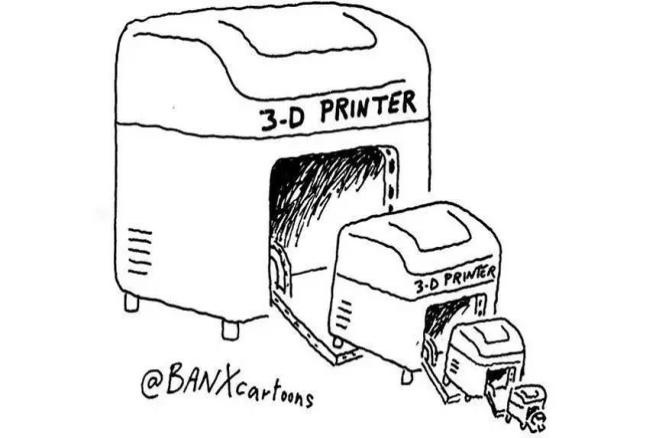
\includegraphics[scale=1.3]{img/C5/5-5/4.png}
\end{figure}

\begin{figure}[H]
	\centering
	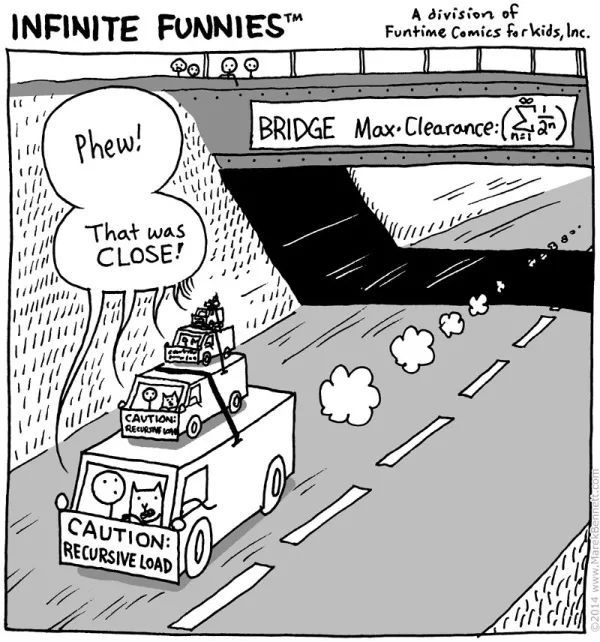
\includegraphics[scale=0.6]{img/C5/5-5/5.png}
\end{figure}

\mybox{无限递归}

\begin{lstlisting}[language=Python]
def tell_story():
	print("从前有座山")
	print("山里有座庙")
	print("庙里有个老和尚和小和尚")
	print("老和尚在对小和尚讲故事")
	print("他讲的故事是:")
	tell_story()

def main():
	tell_story()

if __name__ == "__main__":
	main()
\end{lstlisting}

\begin{tcolorbox}
	\mybox{运行结果}
	\begin{verbatim}
从前有座山
山里有座庙
庙里有个老和尚和小和尚
老和尚对小和尚在讲故事
他讲的故事是:
从前有座山
山里有座庙
庙里有个老和尚和小和尚
老和尚对小和尚在讲故事
他讲的故事是:
...
\end{verbatim}
\end{tcolorbox}

递归函数一般需要定义递归的出口,即结束条件,确保递归能够在适合的地方退出。\\

\mybox{阶乘}

\begin{lstlisting}[language=Python]
def factorial(n):
	if n == 0 or n == 1:
		return 1
	return n * factorial(n-1)

def main():
	print("5! = %d" % factorial(5))

if __name__ == "__main__":
	main()
\end{lstlisting}

\begin{tcolorbox}
	\mybox{运行结果}
	\begin{verbatim}
5! = 120
\end{verbatim}
\end{tcolorbox}

\begin{figure}[H]
	\centering
	\begin{tikzpicture}[]
		\draw (0,0) rectangle (3,1.5);
		\draw (3,-2) rectangle (6,-0.5);
		\draw (6,-4) rectangle (9,-2.5);
		\draw (9,-6) rectangle (12,-4.5);
		\draw (12,-8) rectangle (15,-6.5);

		\draw (12.75,-10.75) rectangle (14.25,-9.25);
		\draw (9.75,-8.75) rectangle (11.25,-7.25);
		\draw (6.75,-6.75) rectangle (8.25,-5.25);
		\draw (3.75,-4.75) rectangle (5.25,-3.25);
		\draw (0.75,-2.75) rectangle (2.25,-1.25);

		\draw (1.5,0.75) node {$ factorial(5) $};
		\draw (4.5,-1.25) node {$ factorial(4) $};
		\draw (7.5,-3.25) node {$ factorial(3) $};
		\draw (10.5,-5.25) node {$ factorial(2) $};
		\draw (13.5,-7.25) node {$ factorial(1) $};

		\draw (13.5,-10) node {$ 1 $};
		\draw (10.5,-8) node {$ 2 $};
		\draw (7.5,-6) node {$ 6 $};
		\draw (4.5,-4) node {$ 24 $};
		\draw (1.5,-2) node {$ 120 $};

		\draw[->] (3,0.75) -- (4.5,0.75) -- (4.5,-0.5);
		\draw[->] (6,-1.25) -- (7.5,-1.25) -- (7.5,-2.5);
		\draw[->] (9,-3.25) -- (10.5,-3.25) -- (10.5,-4.5);
		\draw[->] (12,-5.25) -- (13.5,-5.25) -- (13.5,-6.5);

		\draw[->] (12.75,-10) -- (10.5,-10) -- (10.5,-8.75);
		\draw[->] (9.75,-8) -- (7.5,-8) -- (7.5,-6.75);
		\draw[->] (6.75,-6) -- (4.5,-6) -- (4.5,-4.75);
		\draw[->] (3.75,-4) -- (1.5,-4) -- (1.5,-2.75);

		\draw (4.5,1) node {$ 5 * factorial(4) $};
		\draw (7.5,-1) node {$ 4 * factorial(3) $};
		\draw (10.5,-3) node {$ 3 * factorial(2) $};
		\draw (13.5,-5) node {$ 2 * factorial(1) $};

		\draw (11,-10.5) node {$ 2 * 1 $};
		\draw (8,-8.5) node {$ 3 * 2 $};
		\draw (5,-6.5) node {$ 4 * 6 $};
		\draw (2,-4.5) node {$ 5 * 24 $};
	\end{tikzpicture}
	\caption{阶乘}
\end{figure}

\mybox{斐波那契数列(递归)}

\begin{lstlisting}[language=Python]
def fibonacci(n):
	if n == 1 or n == 2:
		return 1
	return fibonacci(n-2) + fibonacci(n-1)

def main():
	n = 7
	print("斐波那契数列第%d位:%d" % (n, fibonacci(n)))

if __name__ == "__main__":
	main()
\end{lstlisting}

\begin{tcolorbox}
	\mybox{运行结果}
	\begin{verbatim}
斐波那契数列第7位:13
\end{verbatim}
\end{tcolorbox}

\begin{figure}[H]
	\centering
	\begin{tikzpicture}[
			level distance=2.4cm,
			level 1/.style={sibling distance=6cm},
			level 2/.style={sibling distance=3cm},
			level 3/.style={sibling distance=2cm}
		]
		\node {$ f(5) $}
		child {
				node {$ f(3) $}
				child {node {$ f(1) $}}
				child {
						node {$ f(2) $}
						child {node {$ f(0) $}}
						child {node {$ f(1) $}}
					}
			}
		child {
				node {$ f(4) $}
				child {
						node {$ f(2) $}
						child {node {$ f(0) $}}
						child {node {$ f(1) $}}
					}
				child {
						node {$ f(3) $}
						child {node {$ f(1) $}}
						child {
								node {$ f(2) $}
								child {node {$ f(0) $}}
								child {node {$ f(1) $}}
							}
					}
			};
	\end{tikzpicture}
	\caption{递归树}
\end{figure}

\mybox{斐波那契数列(迭代)}

\begin{lstlisting}[language=Python]
def fibonacci(n):
	f = [0] * n
	f[0] = f[1] = 1
	for i in range(2, n):
		f[i] = f[i-2] + f[i-1]
	return f[n-1]

def main():
	n = 7
	print("斐波那契数列第%d位:%d" % (n, fibonacci(n)))

if __name__ == "__main__":
	main()
\end{lstlisting}

\begin{tcolorbox}
	\mybox{运行结果}
	\begin{verbatim}
斐波那契数列第7位:13
\end{verbatim}
\end{tcolorbox}

\vspace{0.5cm}

\mybox{阿克曼函数}

\begin{align}\nonumber
	A(m, n) =
	\begin{cases}
		n + 1             & m = 0        \\
		A(m-1, 1)         & m > 0, n = 0 \\
		A(m-1, A(m, n-1)) & m > 0, n > 0 \\
	\end{cases}
\end{align}

\begin{lstlisting}[language=Python]
def A(m, n):
	if m == 0:
		return n + 1
	elif m > 0 and n == 0:
		return A(m-1, 1)
	else:
		return A(m-1, A(m, n-1))

def main():
	print(A(3, 4))

if __name__ == "__main__":
	main()
\end{lstlisting}

\begin{tcolorbox}
	\mybox{运行结果}
	\begin{verbatim}
125
\end{verbatim}
\end{tcolorbox}

\begin{figure}[H]
	\centering
	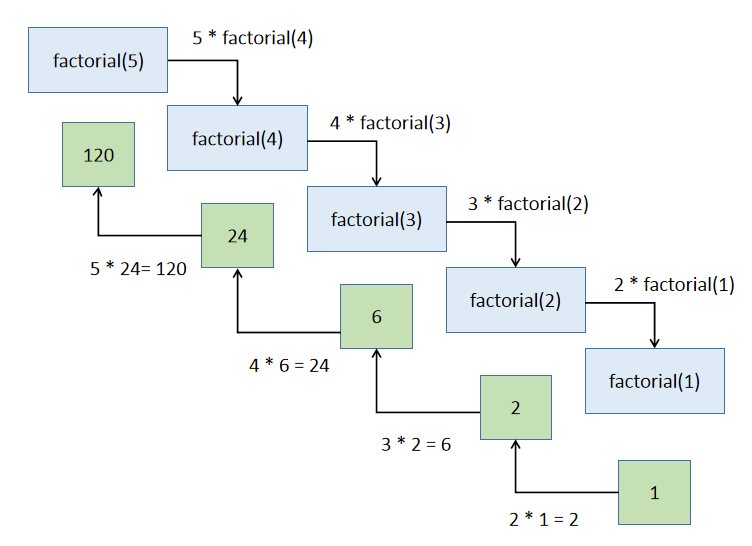
\includegraphics[]{img/C5/5-5/6.png}
\end{figure}

\mybox{汉诺塔}\\

给定三根柱子,其中A柱子从大到小套有n个圆盘,问题是如何借助B柱子,将圆盘从A搬到C。\\

规则:

\begin{itemize}
	\item 一次只能搬动一个圆盘
	\item 不能将大圆盘放在小圆盘上面
\end{itemize}

\begin{figure}[H]
	\centering
	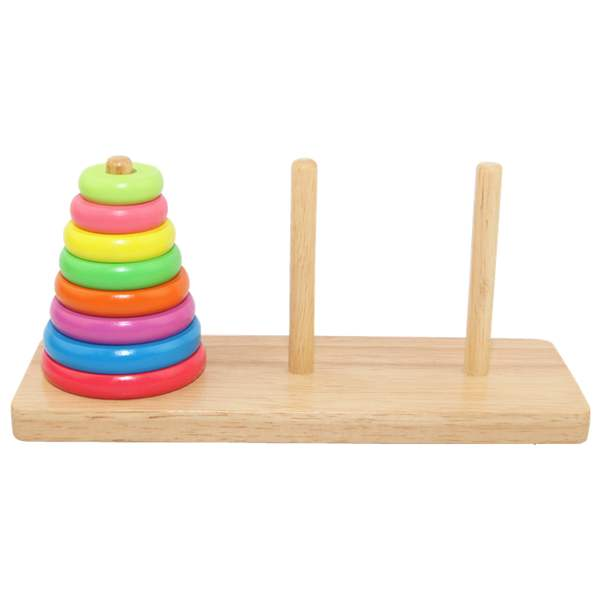
\includegraphics[scale=0.3]{img/C5/5-5/7.png}
\end{figure}

递归算法求解汉诺塔问题:

\begin{enumerate}
	\item 将前n-1个圆盘从A柱借助于C柱搬到B柱。
	\item 将最后一个圆盘直接从A柱搬到C柱。
	\item 将n-1个圆盘从B柱借助于A柱搬到C柱。
\end{enumerate}

\begin{lstlisting}[language=Python]
move = 0			# 移动次数

def hanoi(n, src, mid, dst):
	global move
	"""
		汉诺塔算法
		把 n 个盘子从 src 借助 mid 移到 dst
		Args:
			n (int): 层数
			src (str): 起点柱子
			mid (str): 临时柱子
			dst (str): 目标柱子
	"""
	if n == 1:
		print("%d号盘:%c -> %c" % (n, src, dst))
		move += 1
	else:
		# 把前 n-1 个盘子从 src 借助 dst 移到 mid
		hanoi(n-1, src, dst, mid)
		# 移动第 n 个盘子
		print("%d号盘:%c -> %c" % (n, src, dst))
		move += 1
		# 把刚才的 n-1 个盘子从 mid 借助 src 移到 dst
		hanoi(n-1, mid, src, dst)

def main():
	hanoi(4, 'A', 'B', 'C')
	print("步数 ==> %d" % move)

if __name__ == "__main__":
	main()
\end{lstlisting}

\begin{tcolorbox}
	\mybox{运行结果}
	\begin{verbatim}
1号盘:A -> B
2号盘:A -> C
1号盘:B -> C
3号盘:A -> B
1号盘:C -> A
2号盘:C -> B
1号盘:A -> B
4号盘:A -> C
1号盘:B -> C
2号盘:B -> A
1号盘:C -> A
3号盘:B -> C
1号盘:A -> B
2号盘:A -> C
1号盘:B -> C
步数 ==> 15
\end{verbatim}
\end{tcolorbox}

\newpage